\documentclass[11pt,a4paper]{article}
\usepackage[hyperref]{naaclhlt2019}
\usepackage{times}
\usepackage{graphicx}
\graphicspath{ {./figs/} }
\usepackage{latexsym}
\usepackage{graphicx}
\usepackage{hyperref}
\usepackage{url}

\aclfinalcopy 

\title{Summarizing Congressional Bills}
   
\author{
  \begin{tabular}[t]{c@{\extracolsep{1em}}c}
    Shay Merchant   & {\tt merchants18@students.ecu.edu} \\ 
    Cason White     & {\tt whitecas18@students.ecu.edu} \\
    Dillon Roberts  & {\tt robertsd13@students.ecu.edu}\\
    Jacob Craiglow  & {\tt craiglowj16@students.ecu.edu}\\
  \end{tabular}
} 
\date{}
\begin{document}
\maketitle
\section{Abstract}

Often, individuals have trouble understanding what is going on in Congress, especially when it pertains to our lawmaking process. This group hopes to change that with a summarizer to parse prospective Congressional Bills, along with a Naive-Bayes classifier to assist in sorting those documents which are especially confusing to the average reader.  The approach is to use an API provided by the government to pull down new bills as they appear, then present them in an easy to read fashion for simple browsing, along with any other relevant metadata, like Bill sponsors, along with the requisite classification.  Overall the project is a resounding success, and allows the user to browse newly submitted Congressional Bills ways that are, on average, much easier to understand than the entire length of the Bill. The project also classifies bills with an accuracy rating of around seventy percent, which is fairly good for a Naive-Bayes classifier.

\section{Introduction}
Bills submitted to Congress are long, involved, and confusing to understand.  This project aims to provide a simple and easy method of understanding these documents through mass summarization of bills that have been submitted through congress week by week, as well as a simple classification of these documents into a few easy to understand categories. Our goal is to allow the average user to look at some of the most recent bills that have been submitted, and quickly ascertain whether the bills are especially important, what the content is, and then (within a margin of error) what category the bill falls under, all within a brief span of time. As far as the group members know, nothing similar to this has been created, though there are of course summarization tools that already exist, which makes this tool especially exciting.  Congress.gov has provided an api specifically for downloading bills, which has allowed the group members to grab documents by upload date, which then enables the summarization and classification of large amounts of documents without the creation of an involved scraper or web crawler.  The summarization itself was utilized using the gensim library, which implements a variation of LDA to process the documents in question.  Our classifier uses Naive-Bayes to classify documents into four separate categories, with a current accuracy rating of about seventy percent, which is expected to climb higher as more documents are added to the classifier's corpus.  Congressional Bills can, on average, be made much more understandable through the application of both a programmable summarizer and a Naive Bayes classifier.

\section{Related work}
Milad Moradi’s group worked on a similar program.[2]
Rather than being focused on political documents, Moradi chose to focus on biomedical texts. Like us, Moradi outlines how the challenge they had to overcome was the different diseases and subcategories of biomedical texts which can affect the way a text is formatted. Moradi’s approach was to tackle summarization in 4 steps. Preprocessing, topic extraction, sentence clustering and summary generation. The pros of this approach is that it is concise and relatively simple to implement. The cons could be that a simple approach may take out some important language and context out of the original text to summarize it.  

Anna Kazantseva, and Stan Szpakowicz also had similar work with summarizing short stories.[3] Their team took a unique approach, whereas they made sure their reader knew certain details about the literature they were reading. The pro to this choice is that you are ensuring that your reader has some level of understanding at the end of the summary, even if the summary is less than ideal. The con to this approach is that a reader may have to have an understanding of the document before it’s summarizes, which could potentially contradict the point of a summary.  

The primary focus of NLP research in regards to legal texts has been within the field of paralegal work with a focus on "e-discovery", a  period within the confines of legislative action where the parties involved will gather evidence to support their arguments. The strongest forces within this research has came from the private sector as anyone posing any new advances has a strong financial stake to gain. In the field of politics the primary focus has been on bill success. This is a binary classification task where data is public ally available online which makes it well suited to solve with NLP techniques.

The most often used approach to the problem has been to utilize a machine learning with a neural network. Neural networks have the capacity to identify features about a text which are indicative of categories. Despite historical success of these language models there has been little success in identifying distinct and significant features about text which would indicate success or failure. Rather the most important features, as intuition might lead to, are contextual features such as the bill being supported by a senior committee member or being supported by the majority party.
In [9] Smith, Yano, and Wilkerson defined a baseline algorithm for measuring the likelihood of a bill being passed in the U.S Congress. Some 85\% of bills do not get passed, and nearly 90\% of bills that are recommended by a committee shall pass. The authors incorporated these findings with the application of linear regression based off of a bill's feature vectors.

In [9] Smith, Yano, and Wilkerson engineered a list of 11 basic measures which were centered around answering questions. These features specifically were found to be more telling than textual analysis for predicting a bill's classification into success or failure. Many of these measures had high prevalence across the set of data which does create some ambiguity in measuring their impact, as they noted.

In their approach [9]S, Y, and Wilkerson also applied 4 categories of bills to reduce prediction error. They differentiated bills into categories regarding trivial issues, technical changes to current laws, recurring issues, and important urgent issues such as the 9/11 terrorist attacks. Using this approach they were able label the data and utilized the 3 most commonly occurring categories of bills which were trivial, recurring, and important, to achieve an accuracy of of 83\% across prediction tasks. However, it was was found that this only produced a marginal improvement upon their baseline for prediction, but could act as a substitute in place of the originals.

The authors also viewed the data set in a bag-of-words representation with unigrams for text and bigrams for titles. With this they were able to create a model that outperformed predictions using a categorical model and a proxy vote model. They were able to deduce from this model that legislators often create bills with the expectation of their failure as a means of providing discussion for the issues that go along with them. Some bills also were found to have died for the fact that they were combined into larger, more encompassing bills.

The data itself has associated role call or voting information for which our experiment was unable to make use of. However, it is worth noting that the unigram and bigram views of data being able to discern features relating to any classification task were successful. The fact that the bag-of-words representation model surpassed that of the other models of the labeled data showed that the text itself held more data than most other features.

Nay[8] hypothesized that textual features about a data could be used to discern the probability of a bill's success. Their approach incorporated the word2vec algorithm. With this approach they were able to predict a probability of pass or failure with a high degree of accuracy. Ensemble learning methods were also applied in the form of random forests and GLMs. Along with this they also utilized a logistic regression to meta-learn from the outcome vector.

What was found of all the approaches proposed was that the combined power of word2vec with the ensemble learning created a a model with an AUC of 0.96 and MeanBrier score of 0.021, which showed the model's success. As with the previous experiments with the task and data it was found that the sponsor being of the majority political party was a key feature in determining success of a bill. With the success of the model it can be shown that the data is well suited to categorization tasks. As with the previous approach however the data is only labeled in this particular regard, not in a topical sense.

Naive Bayes classification, the algorithm that was elected as driver for our classifier, has been well established in industry and research. One such research from Almaleh, Aslam, Saeedi, and Aljohani integrates naive-bayes in their research to approach the task of classifying job postings and curricula into their respective subject based on produced keywords as part of a larger effort to build a framework to align academic curriculum with industry demands [12]. The results of their research produced a heatmap of course similarity to job demands based off job postings. In their application of Naive Bayes classifier they were able to obtain strong accuracy with a precision of 85\% and recall of 81\%. Although their approach was much more traditional than other modern approaches that integrate neural networks it was nonetheless found to be very effective for its task. Thus it shows that even as a cog in an advanced analysis that Naive Bayes is an effective classification algorithm for labeled data.

Other works have targeted tasks closer to the domain of the subject of government documents in the form of legal documents. This is a well researched task that  Noortwijk, Visser, and De Mulder approached with Naive Bayes in their research[13]. Specifically, they approach the task of document retrieval given a legal concept, which is a type of ontology or higher-level concept extracted beyond any surface level meaning. They introduce not only the novelty but necessity of introducing a robust search that can incorporate search by abstract content for the domain of case law, and how it might be applied beyond that singular domain.

One core challenge inherent to Naive Bayes is the act of obtaining labeled data. The researchers took a novel approach where they utilized positive, and negative examples for deriving document labels. The intuitive weaknesses of this method requiring user expertise are noted, but the researchers anecdotally allude to this mastery being a fairly swift task requiring only a few hours to obtain sufficient mastery, and more importantly a stronger query. Essentially the argument is made that the user would take nearly equal time with traditional searching queries to achieve the same results.

This novel approach demands user input, but how much? The results of their research showed that the upper bounds for creating a query specific enough to be sufficient for the user's target documents were no more than a few dozen. Beyond their initial search, the question inevitably arises of how to reuse this computation? Certainly it is not a stretch that queries need not be constantly reformulated and be somehow applied in meaningful ways to improve the understanding of new documents, which is exactly what the researchers did.

A program, CODAS, was utilized to create a "concept" file and a dictionary file of word use across documents. These files were given as inputs to the classify functionality of the program which was able to assess new documents entered into its database and evaluate their similarity to the "concepts" in relation to the dictionary. While the end product of their research wasn't near perfect it did show an improvement over the simple a priori probabilistic interpretation of the data they used as example.

Overall the novel approach to query formulation by process of specifying a set of similar and dissimilar documents presented a strong concept unlike many other query systems. Its results vindicated its strengths in that regards, particularly its ability to classify new documents. This user-centric approach to building labeled data for classification explored and leveraged the query in a fashion that could likely lead to further innovation in the field of document classification in a way that encompasses something intrinsic yet abstract from the stored data.

Naive Bayes classifiers have been observed to be accurate with a variety of tweaks to their their nuances. Viegas, Goncalves, Martins, and Rocha [14] introduce changes to the model within their research to address the issues of real world document collections that are difficult to address in the pure configuration. Specifically they relax the independence assumption of a Naive Bayes model and explore Lazy Semi-Naive Bayes models. This change to the model also introduces new computational time penalties, however the authors explored a parallel application of their models that was able to provide speedups of up to 63.36 times.

The research introduces 3 models of lazy semi-NB classifiers: TAN, SP-TAN, and LSPTAN. These all are implementation of an alteration to a Naive Bayes model that produces a Tree Augmented Naive Bayes (TAN) model. This model utilizes the constraint that attributes of the model may depend on only 1 other attribute, in addition to the class. The SP-TAN, or Super Parent TAN is a variation of TAN that introduces the concept of a super parent and favorite child: super parents are attributes for which become the dependency of "orphan" attributes which are purely class dependent and favorite childs are a singular child of the super parent which produces the most improvement in accuracy for the model. The final alteration the researches made to this model address the high cost computation issues of the SP-TAN model. Their change was to enable a lazy super parent model or LSPTAN.

Beyond the integration of lazy evaluation the researchers also utilized 3 novel strategies to exploit different approaches to building a LSPTAN model. They pursued a strategy that forgoes selecting the favorite children to analyze the impact of only selecting the best super parent, another that selects a super parent for each class and allows for it to select any number of favorite children such that the dependencies between the attributes of each class, and finally an approach that evaluates favorite children and super parents in tandem which enables attributes which strictly increase the probability of a document to fall into a class are included in a the model.

The researchers implemented and tested these results on a multitude of large public data sets commonly used for testing including Reuters, ACM-DL, 20 newsgroups, Universities, and Reuters Corpus Volume 1. From their tests they found that their models had success compared to the popular modern models of SVM and KNN implementations and subsequently over traditional Naive Bayes. In some cases their model outperformed its competing algorithms by 18.5\%. These results definitively show that Naive Bayes can, with modification, still serve as the basis for a strong approach in many classification problems in modern day Natural Language Processing.

\section{Methods}
As stated earlier, we are striving to make legislation more approachable. We have decided that the best way is to directly view the legislation itself. Politicians employ rhetoric and lie however, this is the word of the law. 
\newline\indent The words these documents contain will come to directly affect every citizen in the country. It is best to view them directly. However, they are almost deliberately padded and fluffed. Hidden behind a wall of jargon. This is an obvious job for NLP tools. There are a few different parts to project that we will discuss here. First we will detail the tools we use to accomplish this. 

\subsection{Tools we used}
The tools we have utilized were mostly a combination of gensim's 
 \href{https://radimrehurek.com/gensim/summarization/summariser.html}{TextRank summarizer} and data.gov's
 \href{https://api.govinfo.gov/docs/}{govinfo api}.
 Gensim's textrank summarizer provided most of what we needed for this project.  It was easy to understand, had a plethora of options, and most importantly, was fairly simple to implement.  
 \newline\indent One needs only to provide a ratio, indicating how large the summary needs to be in relation to the larger piece of text (in our case, this was the bill), and the group was well on the way to providing consise, readable summaries.  The only real issue was that the summaries made tended towards word salad with larger bills, indicating that we needed to try a variety of techniques to split the bills into smaller chunks for the summarizer to process.
 
 Other notable tools start with Python's local JSON library. Our documents come in a json object from the API, so placing these into a local object made data extraction very convenient indeed. We also made extensive use of numpy in both Gensim's textrank summarizer and our Naive-Bayes classifier. Asciiplotlib (which is in turn derived from mathplotlib) was used for data visualization as an improvement to the project.

\subsection{Data Gathering}
 We decided it would be best to be able to gather documents within the application. Somewhat fortunately, within the last couple years the US Government has implemented a useful API. This allows us to gather our data inclusively. We felt this adds much to the convenience of the application. The point of the application is to be something you can open and immediately expand your political knowledge. 
 \newline\indent Because of this, we made this a crucial part of our project. While there is not a method to add your own documents, we do allow our naive bayes classifier to be trained on whatever documents you like. As such, you are free to customize this as you wish.To include this important functionality to our application we capture bills matching date criteria from an API at https://api.govinfo.gov/collections/BILLS/. The API is maintained by the government and contains valuable information about the logistics of each political document as well as the document itself. We are able to give a specific span of time to the API and receive all political documents that it has access to. These come in the form of JSON objects with metadata pertaining to each document. If you were to call this API on an older document, you would notice that you would not be able to. This API was created fairly recently. And lots of documents were added at one time. So while you are able to get documents from years back, you will want to pay special attention to the “dateIssued” value of the received JSON file. This value will give you the proper date of the bill. These documents then get pumped into our summarizer. This process is remarkably quick unlike most things in the government. You will be able to grab years worth of documents in just a moment.

\subsection{Tokenization}
As with most of NLP, a mantra to keep in mind is “Garbage in, Garbage out.” So we took care to clean our documents. Our summarizer is based on assigning an importance value to sentences and thus we have to be sure to leave in periods and other punctuation. Removing these will essentially break the algorithm so special care must be taken to avoid this. To handle this we create a bag of words seperately for our naive bayes classifier and keep a copy of the original cleaned document for our summarizer. 
\newline\indent   One interesting aspect of congressional legal documents is the different stop words that must be taken into account for good classification and summarization. Several words become exceedingly common. "Legislation", "president", "congress", among several others becoming what we'd classify as garbage or jargon. Along with these, the documents are not very clean and contain many programmatic artifacts such as “[document]”, “head”, “script”, etc. These can cause serious misclassifications and must be removed in preprocessing. We also remove traditional stopwords such as “and”, ”of”, ”the”, etc. After this we construct a bag of words representation of each individual 
document to feed to our classifier. 

\subsection{Classification}
After grabbing the documents in question, stop word removal, and tokenizing the data we then pipe a bag of words to the Naive Bayes classifier.  We have built a model with four different classifications. Firearms/Explosive, Government/Political, Environment/Weather, Healthcare/Medicine/Welfare bill. These four categories were chosen as together they cover a broad spectrum of the political sphere. 

Firearms pertains to legislation regarding firearm and ammunition usage.This can also be used for ordinance and taxation as well. As well as  purchasing rights. 

The political label is a nebulous one that consists of legislation affecting the state of our legislative, judicial, and executive branches. We always made this encompass change to state rights as rare as they are. This includes everything from salary adjustments to procurement of naval vessels in international waters. 

The Environmental label consists of legislation dealing with pollution standards and wildlife. This can also include things like national park budgeting and other forms of preservation. 

Finally, the medical label Simply deals with anything regarding prescriptions. This was very important to us in light of the timing of our project. This can include drug trade, medicare, or general insurance. Even state or federal guidelines. It is another very nebulous topic however, extremely important in our current political climate. 

To train our model, eighty bills and joint resolutions occurring in the past year were hand annotated and classified into one of these four categories. As a proof of concept we found twenty training docs for each classification. Bills can vary wildly in length so special care was taken to curate bills of similar lengths for each category. Initial failure to do so resulted in false classifications. 

This is a much smaller data set than we would like to train on. However, between hand annotation, time constraints, and there being very little data on where each bill would fall we felt this was as much as we could realistically accomplish. After training we can feed our classifier new documents as we like and of our choice. However, care should be taken to ensure the training data is balanced. We also made sure each bill was very recent. This is important as topics and language can change wildly as time progresses and congress members rotate out. Failure to do this cold result in false classifications in our current political climate and would be detrimental to the usefulness of the project. 

After cleaning and tokenizing our documents they are sent as a bag of words to the Naive Bayes classifer. Our Naive Bayes classifier is trained on initialization due to the small amount of training data. However this is easily saved and loaded once the project scales. Upon call we compute the log posterior of the document and labels and return the most probable classification. 

Our current Naive Bayes model was then tested and found to have an accuracy of 75\% (see 6). Our test data consisted of bills gathered from a similar time and were also hand annotated. We surmise that this accuracy is simply a lack of training data. As all our documents are bills, much of the language is political jargon and very similar from document to document. With more data our classifier will be able to properly weight the distinguishing terms. Given our small training data set we thought four classifications should suffice as proof that Naïve Bayes is feasible for the purpose of bill classification.

\subsection{Summarizing}
Following classification we then create a multi-sentence summary of the documents. This is accomplished by Gensim’s summarize function. Gensim uses the TextRank algorithm initially presented by Rada Mihalcea and Paul Tarau of the University of North Texas. 
\newline\indent Textrank is a graph-based ranking algorithm that sets sentences as nodes on a graph. It takes the degree of each node as a rank with the highest ranking sentences being most important. This is determined by similarity to other sentences. The sentence classified as similar enough to another sentence gains an edge connecting the two. Essentially, the sentence most similar to the most sentences in the document is considered the most important sentence and thus will have the highest degree. Then the summary is based off of the connected vertices. 

Gensim's summarize function takes two parameters. The document and a ratio. We set a ratio of 0.75. This ratio essentially controls the proportion of summary sentences to document sentences. A proportion of three-fourths gives us a solid summary while still cutting potentially unnecessary information. This preserves our initial mission statement. Due to the nature of gensim’s TextRank summarization algorithm there is no need to train any models as it is unsupervised. Much of the work lies in proper preprocessing of the data and tuning of the pre-existing algorithm in order to best suit the document. We then display the bill metadata, classification, and the summary.

\subsection{Git Links and Directory Discussion}
Here we will break down our git methodology and project structure. 

We opted for the basic git workflow with a single branch and communicating our changes in our tri-weekly meetings. Our directory structure is similarly simple. All of our code is located in the src/classifier folder. This contains the Naive Bayes, user interface, API, and summarizer code. Currently it also contains our training and test data. However, this will be moved to our data folder promptly. The pub folder contains all textual project information including the readme.md as well as our previous progress reports and initial proposal. 

\begin{enumerate}
    \item \href{https://gitlab.com/Merchant89/b/-/blob/master/src/Classifer/UserInterface.py}{User Interface} - Driving code. Gives the user the option of viewing bills or joint resolutions. It then asks the user what date range they would like to view. As well as a shortcut to the past weeks.
    \item \href{https://gitlab.com/Merchant89/b/-/blob/master/src/Classifer/WebsiteInfoGetter.py}{API} - WebsiteInfoGetter is built to query the https://api.govinfo.gov/collections/BILLS/ API for a user specified set of bills. The user will ask for a specific range of dates. 
    \item \href{https://gitlab.com/Merchant89/b/-/blob/master/src/Classifer/ResolutionSummarizer.py}{Summarizer} - This contains the code built to summarize either a bill or a joint resolution. This also runs the Classifier on the document. 
    \item \href{https://gitlab.com/Merchant89/b/-/blob/master/src/Classifer/NaiveClassifier.py}{Naive Bayes Classifier} - This is the file containing all of the Naive Bayes code including training, testing, and querying.
    \item \href{https://gitlab.com/Merchant89/b/-/tree/master/src/Classifer/train}{Training Data} - Currently in src/classifier folder but will be moved to data presently.
    
\end{enumerate}
\section{Data}

When choosing our data set, we made sure that our data would be readily accessible and plentiful. A personal requirement for the data set, was our data had to be something that is relatable, something interesting, and something that could matter to a lot of people. The data that we decided for our program to run on was congressional-records and bills from the United States Congress.[4] \\
\indent The LDA algorithm is an unsupervised learning algorithm and thus does not require a training set persay. However, there will be testing done on small increments of a day's transcript throughout the length of the project. This data is freely available for download from congress.gov and is the main focus of our work. Its contents are records of politicians discussing issues stored in PDF format. This can be parsed using pdfminer, a Python library.

The progress in our dataset is that our group is using data compiled from congressional records.[4] The congressional records have been recorded, and are accessible for every week day since 1994. This gives us roughly 6,760 documents to access. Each of these documents range in size depending on the amount discussed or the amount done in congress that day. On average each document is around 150-300 pages in length. 
\newline\indent This larger document is also available in many separate, smaller sub-categorical text documents. The sub-categories are daily digest, extension of remarks, House and Senate. The daily digest provides an extremely brief and undescriptive synopsis of the events that occured that day. The extension of remarks is just an extension to remarks on the senate floor given to the recorder after the event has occured. 
\newline\indent Lastly, the House and Senate contain our main focus and contain the data of all the events that occured that day in detail. 

Our original intent for these documents was for our program to be able to access any one of these documents and summarize it. Once it became clear this was beyond the scope of our planned summarizer, we narrowed our focus on specific portions of the original full documents. We decided to focus on specific sub documents we deemed important. This allowed our summarizer to perform a much better job at summarizing the text. Because these documents were also available as text, it also allowed us to disregard the use of pdfminer, and use the text documents directly. Lastly, we will be experimenting with summarizing the specific subsection of Public Bills And Resolutions and Private Bills and Resolutions. These seem like the most viable source to summarize as they are split by the header "H.R" followed by the bill's resolution number. This would viable in the sense, we can split each of the bill's and resolutions easily, summarize them, and present them to the user. 
Once we accomplish the summarizing of Bill Resolution's, we may use the larger data set to experiment with other forms of summarizing, such as keyword summarizing or summarizing larger bodies of political text with visualizations.  
\section{Tools expanded}
This section we'll go over a more in depth explanation of the tools we used in executing our summarization program.
\subsection{Tools for corpus and data retrieval}
The tool we decided was the most efficient method to use to acquire our corpus is an API. This API is provided by the government on their govinfo website[10]. The first step in utilizing the API website is requesting an API key from their request page. The figure below displays what this request website looks like.
\newline\newline
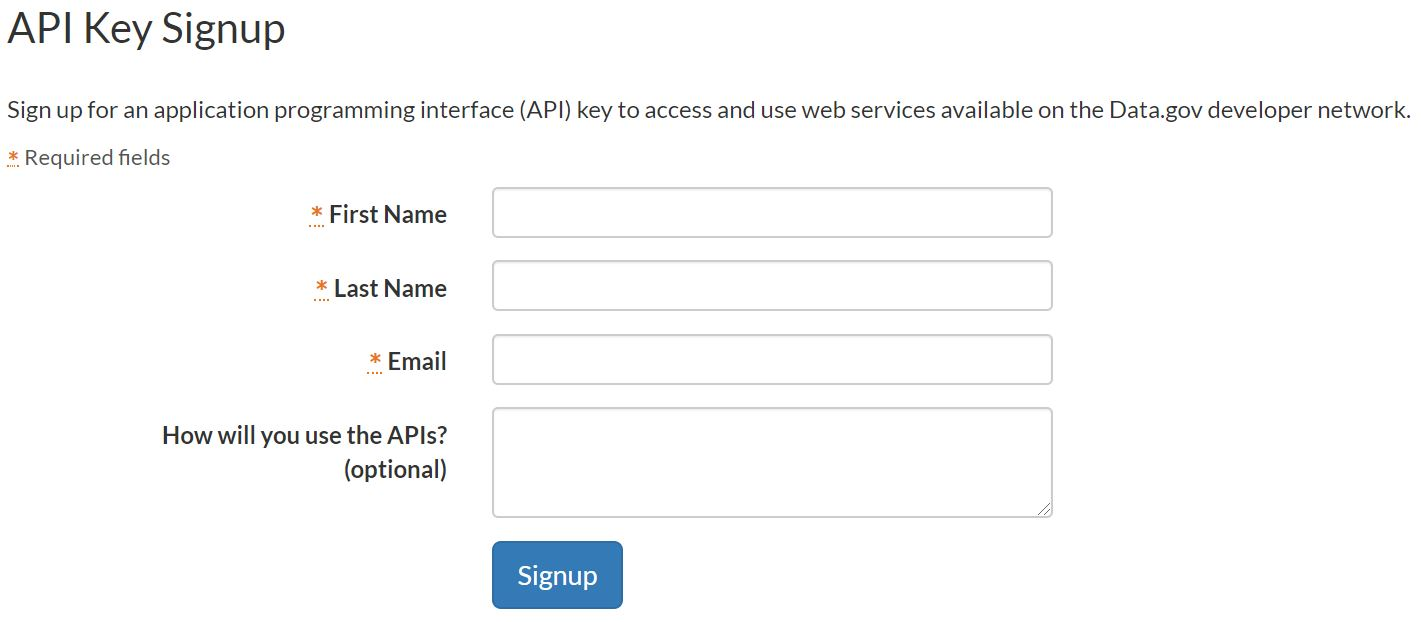
\includegraphics[scale=0.32]{figs/Apikey.jpg}
\newline\newline
After receiving the api key from the govinfo website our next step to receive our corpora was to generate an API URL. A figure of what this URL generator looks like can be seen below.
\newline\newline
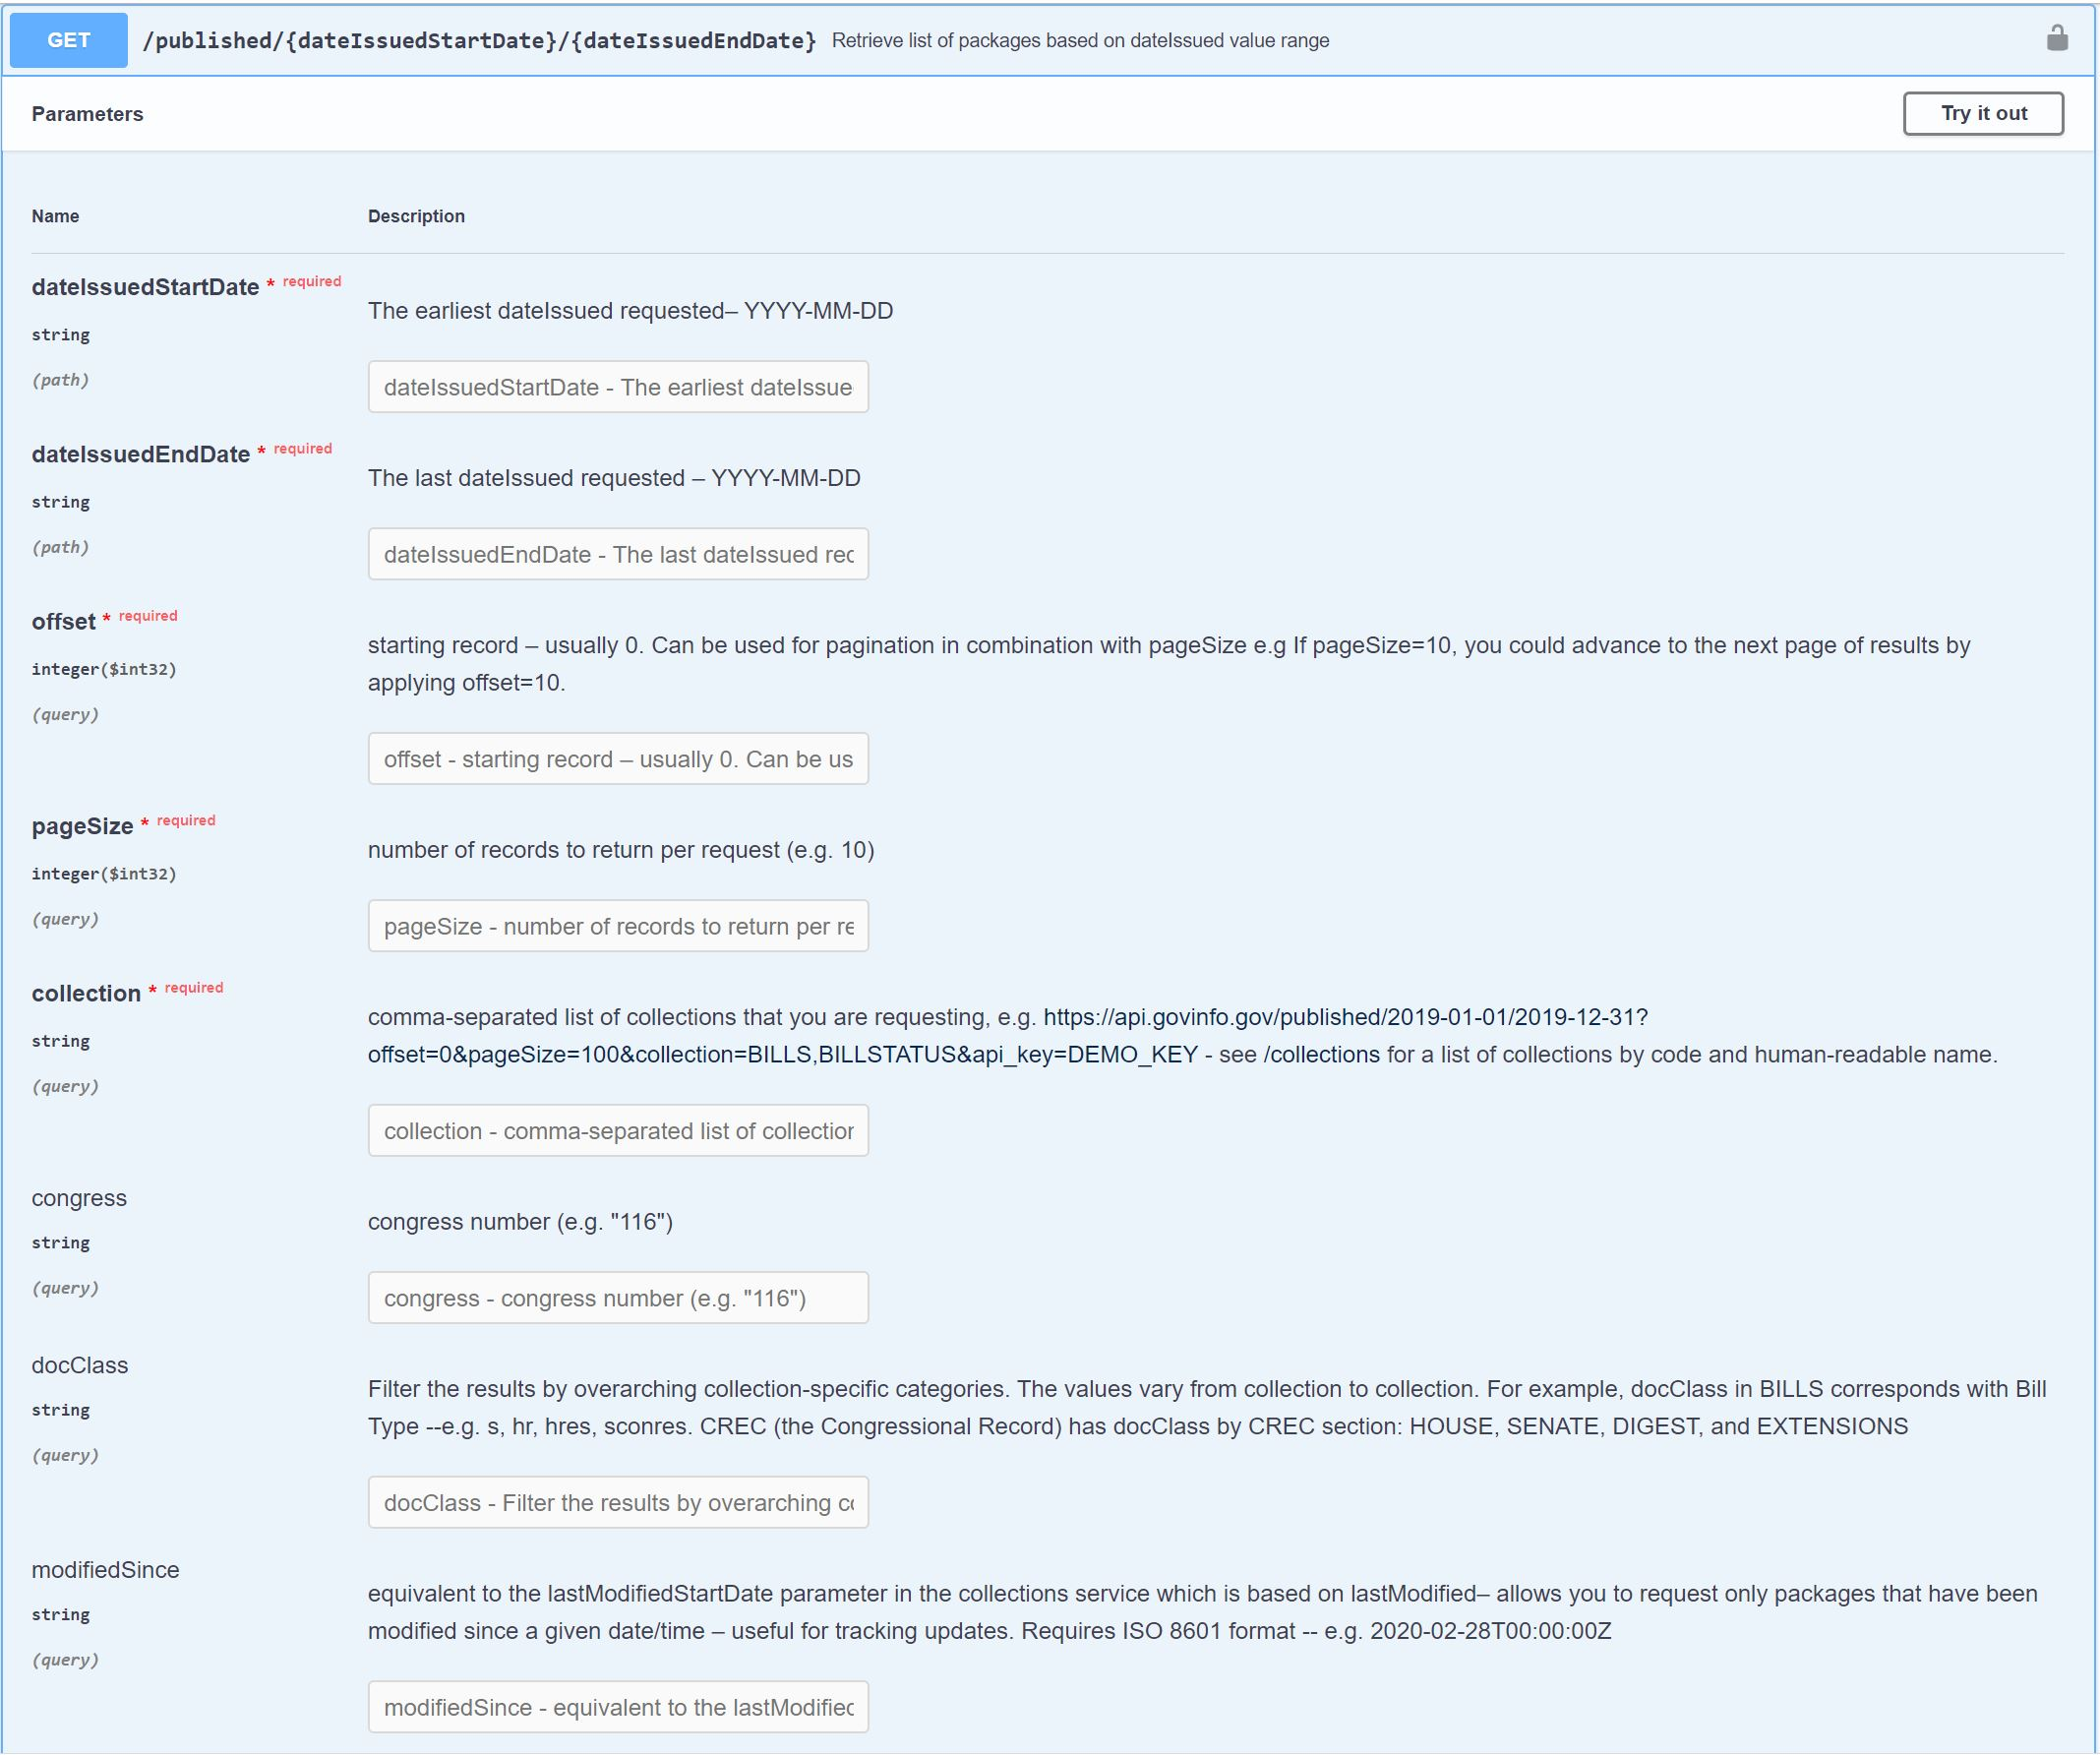
\includegraphics[width=8.1cm, height=9cm]{figs/Urlgeneration.JPG}
\newline\newline
After filling in the fields below you can get a URL like this one:
\newline
\newline
\noindent
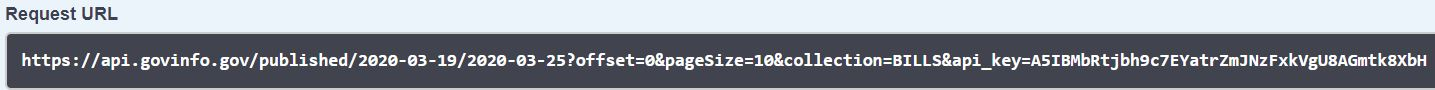
\includegraphics[width=8.7cm, height=1.1cm]{figs/URL.JPG}
\newline
\newline
\noindent
Taking this URL you can modify date ranges and document types to pull a JSON file that holds bill.txt files and bill specs such as congressional number, section number, bill title, issue date, bill sponsor and bill sponsor political party. 
\subsection{Tools for preprocessing}
There are many libraries for assisting with preprocessing in the Python language. Like our summary we decided to use Gensim to handle our preprocessing.The specific tools or functions we decided to implement within Gensim are:
\newline\newline
\noindent-\textbf{remove\_stopwords():} This function removes common stopwords such as "the", "but", "than" etc. Below is an example pulled from Gensim's website[5] of how this works.
\newline
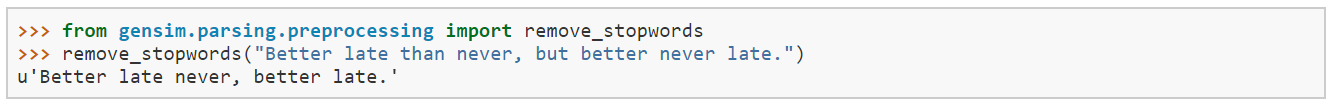
\includegraphics[width=8.30cm, height=1.2cm]{figs/remove_stopwords.PNG}
\newline\newline
-\textbf{strip\_numeric():} This functions removes any numeric strings from the text.
\newline\newline
-\textbf{strip\_short():} This function removes strings that are less than or equal to the parameter length provided. Below is an example pulled from Gensim's website[5] of how this works.
\newline
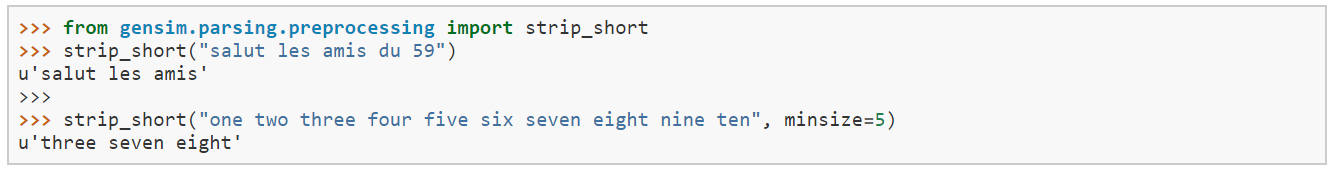
\includegraphics[width=8.2cm, height=1.8cm]{figs/strip_short.PNG}

\subsection{Tools for summary}
-\textbf{summarize():}
Our bill summaries utilize Gensim's summarize() function. This summary is creates an extractive summary rather than an abstractive summary. Essentially Gensim's ranks the most important sentences by their top word's and apphends them as a summary. Below is an example pulled from Gensim's website[5] of how this works. 
\newline
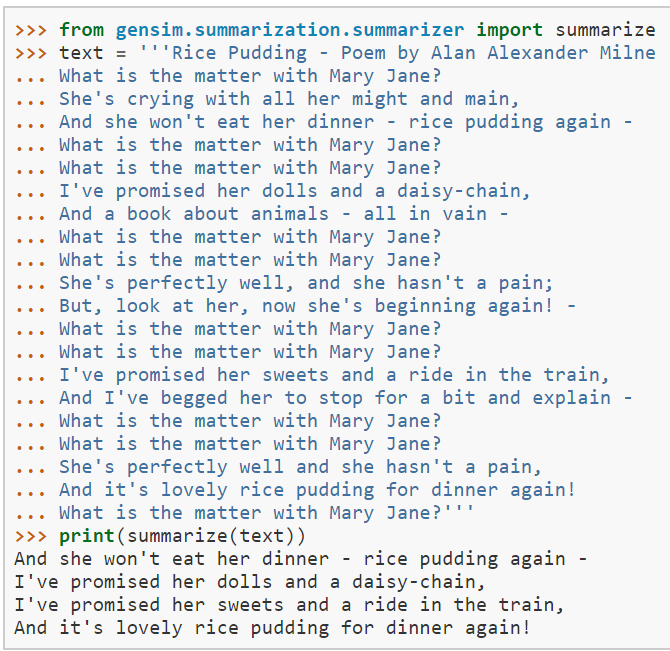
\includegraphics[scale = .68]{figs/summarizer.PNG}
This summarize function contain's a word to summary ratio that we have modified for different bill lengths to minimize the overall length of the bill summary as much as possible.

\subsection{Tools for Data Visualization}
For visualizing our data we used the library asciiplotlib. We decided to use this library over the popular library matplotlib due to asciiplotlib's concise and basic bar graph. This gives a quick and basic summary of the top n words of each bill.Below is an example pulled from asciiplotlib's website[11] of how this works.
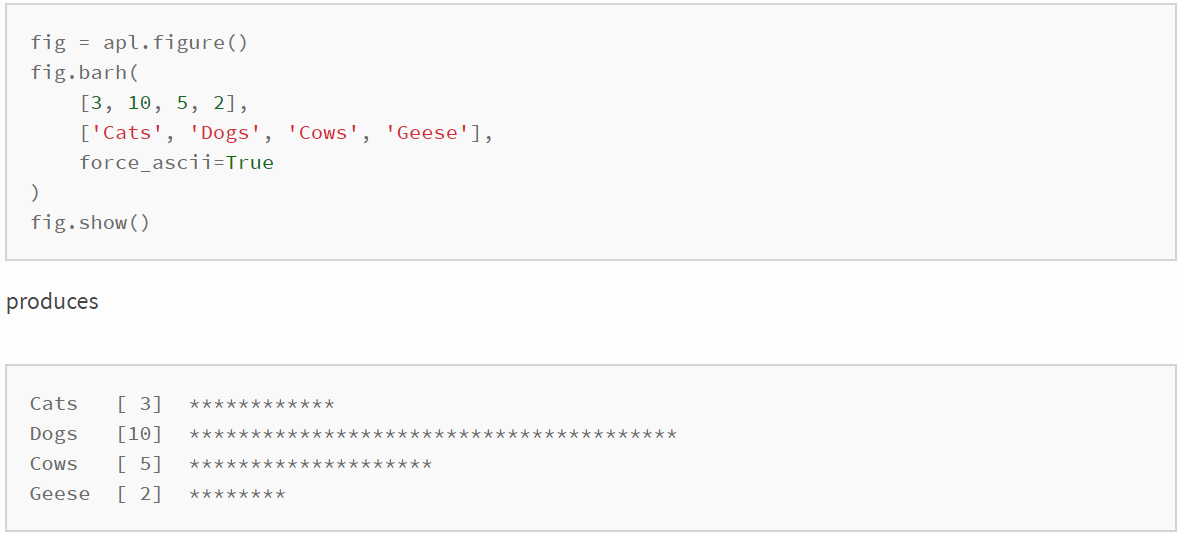
\includegraphics[width=8.1cm, height=5cm]{figs/asciiplot.PNG}
\subsection{Tools for classification}
The tool used for our classifier is a custom Naive Bayes model utilizing four labels that we created. This classifier has many functions we are using for our classifier.

-\textbf{top\_n():} This function return's the top n words within the trained model.

-\textbf{classify():} This function utilizes helper functions to classify a bill into one of four labels. The labels are environmental, firearm, health and government. 

-\textbf{evaluate\_classifier\_accuracy():} This function calculates a rough accuracy of the classifier on a test set of bills.

-\textbf{tokenize\_doc():} This function, while technically a part of preprocessing, is within our Naive Bayes classifier function. This function turns a document into individual tokenized strings.

\section{Data and Results}
\subsection{Classifier}
 We applied Gensim's keyword function to create a bag of words representation of keyword-document frequencies. The tokens which occurred the most as keywords in a set of testing data that consisted of 122 documents showed that the raw data from navigating elements in the XML tree were "dirty", so we ignored the first 14 of them in the infographic and found more meaningful keyword frequencies. We chose to use a small fraction of the corpus as navigating XML trees proves computationally expensive along with keyword generation.
  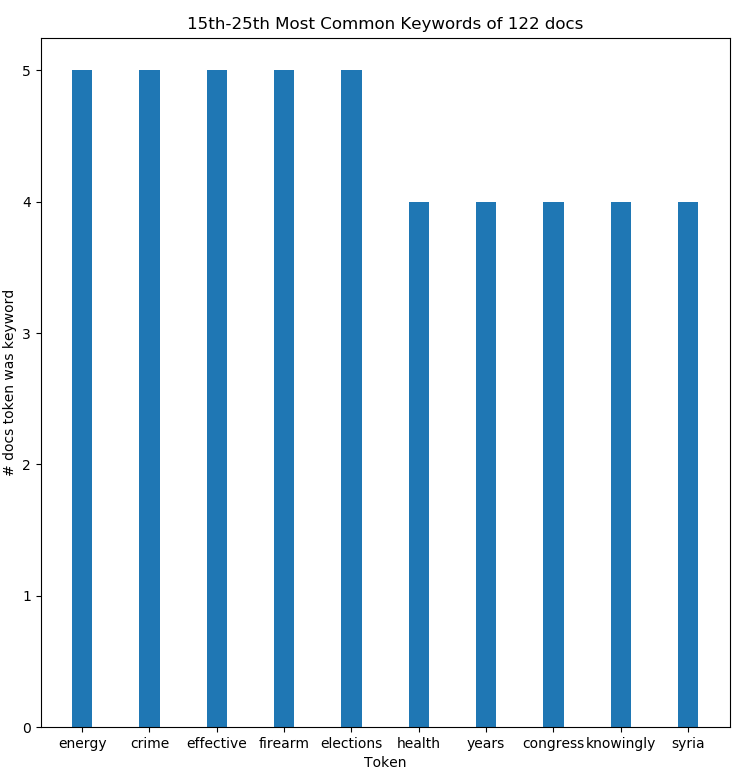
\includegraphics[scale=0.43]{test_kw-mostcommon_15-25}
 This graph represents the 15th-25th most common keywords of 122 documents. From this data we decided to to seperate Bill's into 4 main Bill labels. The labels are environment, health, firearms, and government. Below is an example of the results of the most common keywords being seperated by label. As seen, some words are ambiguous and can be shared by more than one label.
 \newline
 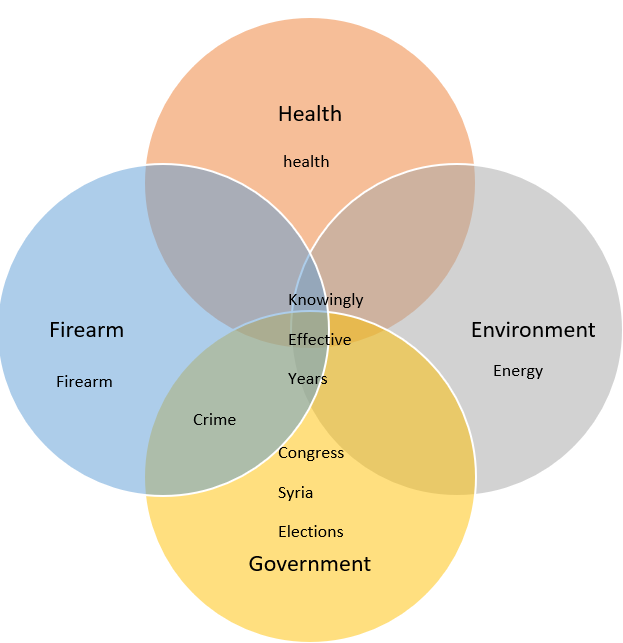
\includegraphics[scale=.74]{figs/Venn.PNG}
  
  Taking our health, firearm, government, and environment labels we set up a classifier using Naive Bayes. This Naive Bayes classifier was then trained with 20, full length Bill's for each label. The training data produced the following top ten keywords for each label. This can be reproduced by running our NaiveClassifier script with the built in function top\_n.
  \newline\newline
  \noindent
  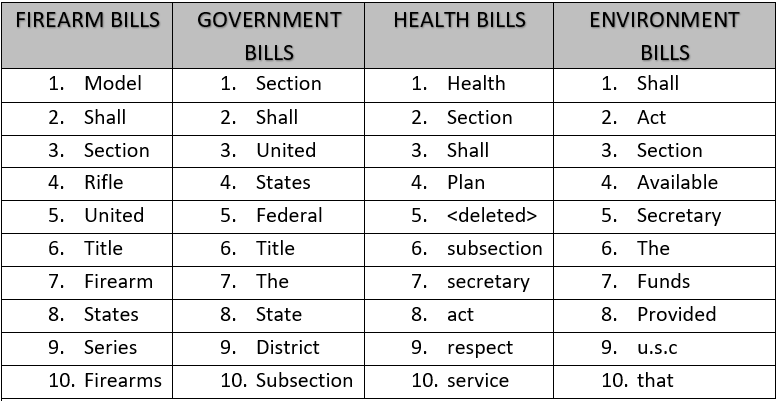
\includegraphics[width=8.2cm, height=5.3cm]{figs/naivetop.PNG}
  \newline\newline
  \noindent
  Running our Naive Bayes classifier on a random selection of Bill's from our 4 catagories, firearm, government, health and environment we were able to achieve an accuracy of 75 percent. This accuracy was calculated by using a simple formula of 
  \[ Label Accuracy = \frac {Labels Correct}{Total Labels} * 100\]
  This can be reproduced using our NaiveClassifier script with the function evaluate\_classifier\_accuracy.This accuracy is also displayed when running our program normally from the UserInterface script.
  Our original goal was to decipher Government Bill's. Here is a success and a failure of our classifier on a couple interesting Bills.
 
 
 \noindent\textbf{Successful classification:}

 \noindent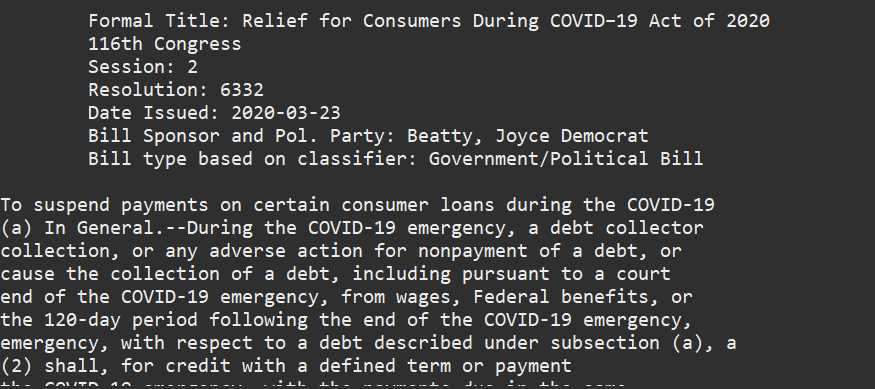
\includegraphics[scale=.54]{figs/Screenshot2.PNG}
 \newlinenewline\noindent\textbf{Unsuccessful classification:}
  \newline
  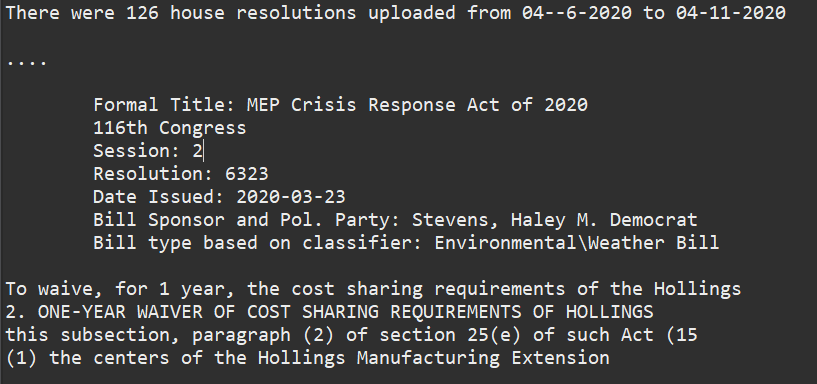
\includegraphics[scale=.57]{figs/Screenshot3.PNG}
  \newline
  
    In the first summary, the classifier is able to classify this Bill as a political Bill, despite the deceptive content of COVID-19 and implications of it being a health bill. The Bill is actually about debt and federal benefits.
  The second Bill is successfully summarized but unsuccessfully classified. The Bill has been classified as a environmental Bill, while the Bill is about giving manufacturing employees the "resources" and ability to work during the COVID crisis. This misclassification is an issue we faced on Bill's that shared many common words with other Bill's. In this case, the Bill referenced resources, which is commonly found in environmental Bills. Both of these examples can be found running our UserInterface script. These two particular Bill's were summarized from the "House Resolutions from this Week" option.
\subsection{Summarizer} Above we showed the results of our classifier, but this is only a small element of our end result. We had to hone Gensim's summarize function to work correctly as some bill's were many pages long. For this we set up a simple check of the bill's length then adjusted the ratio of word to summary in the Gensim function. Below is a chart of the word length to word to ratio that we decided worked the best.
\noindent\newline\newline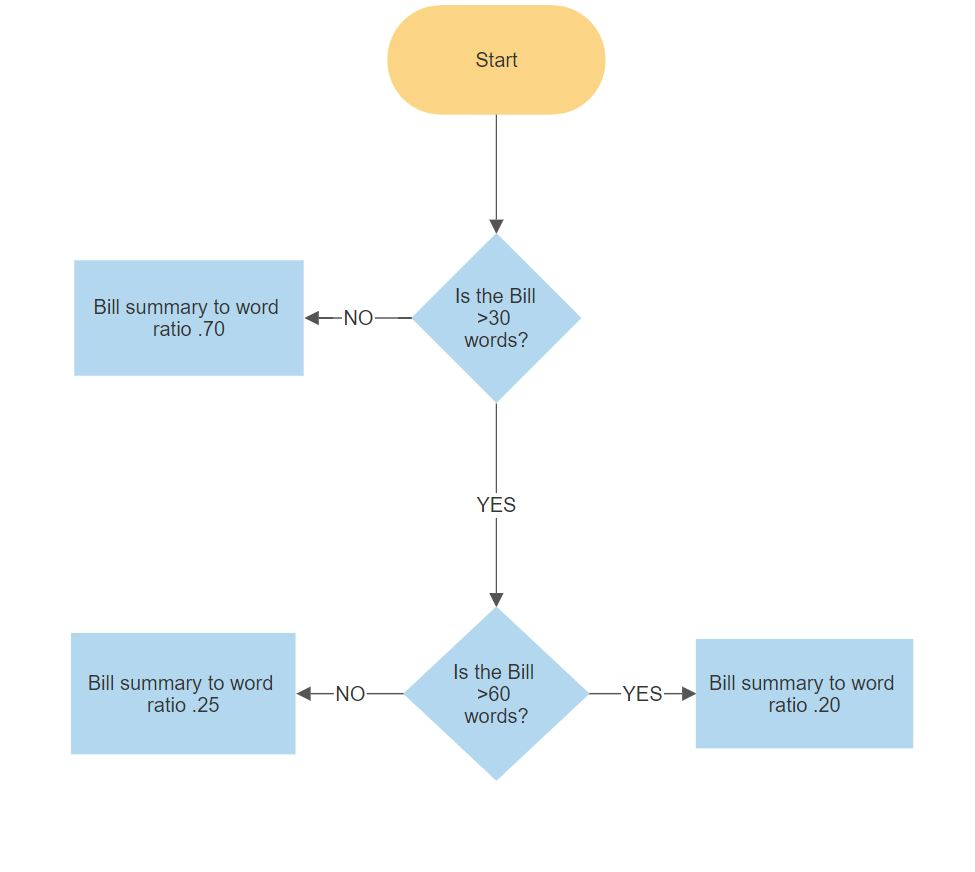
\includegraphics[width=8.8cm, height=9cm]{figs/Flowchart.JPG}
\newline\newline
The end result combined with our classifier and json bill information looked like the figure below.
\noindent\newline\newline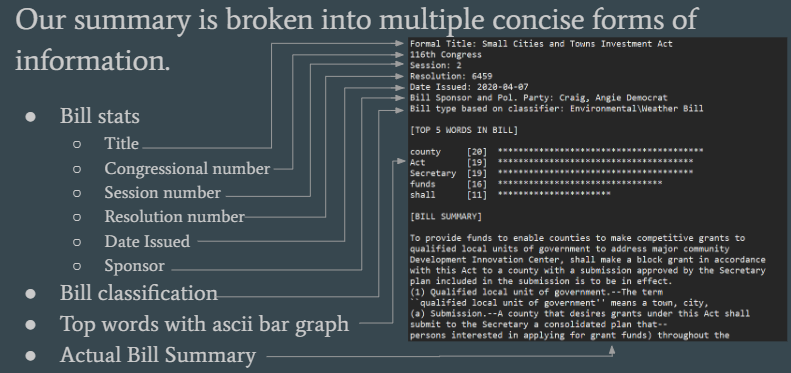
\includegraphics[width=8.2cm, height=5.3cm]{figs/Data.PNG}

\section{Discussion}
As previously discussed in our introduction, we believe most will see the desire for an unbiased news source. Something becoming depressingly clearer as time moves on is that news companies are violently vying for our attention. They resort to sensationalized headlines and a lack of substance. They've also been known to lie and never issue any retractions. A career ending taboo just years ago. 

As such, the clear need for such a project is painfully apparent in these troubled times. Getting your news as close to the source is the difference between drinking from a swift clear mountain stream or a dank stagnant pond. As the news agencies 24 hour cycles tumble on a game of telephone begins that can detrimental to our individual freedoms. Thus being well informed with as unbiased news as you could possibly get is crucial to maintaining one's autonomy in these troubled times.

Removing this filter of bias is crucial and we have succeeded by our standards. The results have been promising. We have achieved both classification and summarization in a relatively short amount of time with relatively high accuracy. While this tool isn't ready to replace any news outlet, this has served as a proof of concept to take note of. 

While our classifier is only showing an accuracy of 75\% currently, we also do not have nearly as much training data as we need. If we refer to the figures of the top ranking words from each label, These labels are indicative of there being several hard hitting and defining terms within the first three labels.Environmental underperformed here but imagine if there was a data set classifying a years worth of bills to train on. 

\section{future work}
This project has been one of passion as much as academia. As such we are constantly thinking of things we would like to do given the proper time and resources. This section will discuss some of these. 

To make this as applicable to as many situations as possible, we could speak for a long time on flexibility. In file type, summary style, and data exporting we leave this to reader however, this project would certainly benefit from it. Specifically a fair amount of legal documents are in a pdf format. This causes many formatting and data cleaning issues and thus we shied away for now opting for text documents through the API. This alone would improve the flexibility of the project. 

The only thing better than data is analytics on the data as I'm sure many would agree. Currently there is none associated with the project as it is slightly out of scope for the average consumer. This is of course a fascinating topic to dive into for anyone in the big data and computer science field and thus features we'd like to add in house. 

One of the simplest and hard hitting analyses that would be simple to add is a distribution of classification and document length over a given window of time. Of course there will be a sharp uptick in medical legislation from January 2020 till ~November 2020 however, how large? Or will politicians use this distraction to tackle another topic? These problems could be solved by a simple time distribution on our classifications.
 
 On the subject of classification, we feel the only think "missing" from the classifier is more training data. Naive Bayes Classification has served us well and as we scale it will only continue to serve us better.
 
 Our four labels were chosen because they really exemplify our modern political climate best. Being that there is a lot of discussion about firearm safety and the century defining tragedy of COVID-19 we added the firearms and medical label. We wanted anyone using this program to immediately see if a bill fell into one of these important topics. However there are so many more topics that could very easily change your day to day life. We will definitely be looking into making this more granular in the future. What we suffer from currently is a lack of training data and will be the first thing to be addressed. 

The summarizer could use tuning. While we certainly have made documents that are surprisingly truncated and readable, these aren't the hard hitting bullet point summary an average consumer would enjoy. There is also a problem or large bills generating large summaries. 

Earlier we introduced you to ratio of the textrank algorithm. We surmise a calculation to dial in this ratio based on the length of the bill would improve performance. However, we opted to focus on other features in our limited window of time. This is indeed a serious problem that runs contradictory to our mission statement of producing digestible truncation and is near the top of the list of desired work.

The method chosen also has the misfortune of not picking up small details that aren't necessarily related to the "main" topic of a bill. A favorite of politicians. 

We believe creating a summarizer/topic model abstract summarizer could solve this problem. By determining the granular topics of a bill and creating an abstract summary that hits on each of these we could possibly build a much more effective summarizer. 

However, this is much more involved. By using preexisting solutions and reqorking them to apply to our problem we have made a powerful statement. We have a firm grasp on the nature of the problem and aim to give anyone a powerful spring board to jump off of in the future. Possibly even ourselves. 
  
  

\clearpage
\section{References}

[1] Los Angeles Times. (2011, June 19). Congress turns bill titles into acts of exaggeration. Retrieved from https://www.latimes.com/world/la-xpm-2011-jun-19-la-na-0620-titles-20110620-story.html 
\newline
\newline
[2] Moradi, M. (2018, November 13). CIBS: A biomedical text summarizer using topic-based sentence clustering. Retrieved from https://www.sciencedirect.com/science/article/pii/S1532046418302156?via=ihub 
\newline
\newline
[3]Kazantseva, A. (n.d.). Summarizing Short Stories. Retrieved from https://www.aclweb.org/anthology/J10-1003.pdf 
\newline
\newline
[4] (n.d.). Retrieved from https://www.govinfo.gov/app/collection/crec/2020/01/01-10/6/{"pageSize":"20","offset":"0"} 
\newline
\newline
[5]GensimLink:
https://radimrehurek.com/gensim/
\newline
\newline
[6]GensimSummarizer:
https://radimrehurek.com/gensim/summarization/summariser.html
\newline
\newline
[7] Mihalcea, R., & Tarau, P. (2004, July). Textrank: Bringing order into text. In Proceedings of the 2004 conference on empirical methods in natural language processing (pp. 404-411).
https://web.eecs.umich.edu/~mihalcea/papers/mihalcea.emnlp04.pdf 
\newline
\newline
[8]Nay J. J. (2017). Predicting and understanding law-making with word vectors and an ensemble model. PloS one, 12(5), e0176999. https://doi.org/10.1371/journal.pone.0176999
\newline
\newline
[9] Yano, T., Smith, N. A., & Wilkerson, J. D. (2012, June). Textual predictors of bill survival in congressional committees. In Proceedings of the 2012 Conference of the North American Chapter of the Association for Computational Linguistics: Human Language Technologies (pp. 793-802). Association for Computational Linguistics.
\newline
\newline
[10]“GovinfoAPI.” Govinfo, api.govinfo.gov/docs/.
\newline
\newline
[11]"Asciiplotlib." https://pypi.org/project/asciiplotlib/
\clearpage
\newline\newline
[12] Almaleh, Ahood & Aslam, Muhammad & Saeedi, Kawther & Aljohani, Naif. (2019). Align My Curriculum: A Framework to Bridge the Gap between Acquired University Curriculum and Required Market Skills. Sustainability. 11. 10.3390/su11092607. 
\newline\newline
[13] https://warwick.ac.uk/fac/soc/law/elj/jilt/2006\_1/noortwijk/noortwijk.pdf
\newline\newline
[14] Felipe Viegas, Marcos André Gonçalves, Wellington Martins, and Leonardo Rocha. 2015. Parallel Lazy Semi-Naive Bayes Strategies for Effective and Efficient Document Classification. In Proceedings of the 24th ACM International on Conference on Information and Knowledge Management (CIKM ’15). Association for Computing Machinery, New York, NY, USA, 1071–1080. DOI:https://doi.org/10.1145/2806416.2806565

\end{document}